\documentclass[UTF8,aspectratio=169,mathserif]{beamer}
\usepackage{ctex}
\usepackage{ulem}
\usepackage{color}
\usepackage{amssymb}
\usepackage{amsmath}
\usetheme{Berlin}
\setbeamertemplate{navigation symbols}{}

\title{6 - 布尔电路}
\subtitle{Boolean circuits}
\author{报告人:许博}
\date{\today}

\begin{document}
	
	\begin{frame}
		\titlepage
	\end{frame}
	
	\begin{frame}{一致与非一致计算}
		\begin{block}{Uniform Computation}
			对不同的输入大小,使用相同的算法。
		\end{block}
		
		\begin{block}{Nonuniform Computation}
			对不同的输入大小,允许使用不同的算法。
		\end{block}
	\end{frame}

	\begin{frame}{目录}
		\tableofcontents
	\end{frame}

	\section{布尔电路和 $\bf P_{/POLY}$}
	\begin{frame}{布尔电路}
		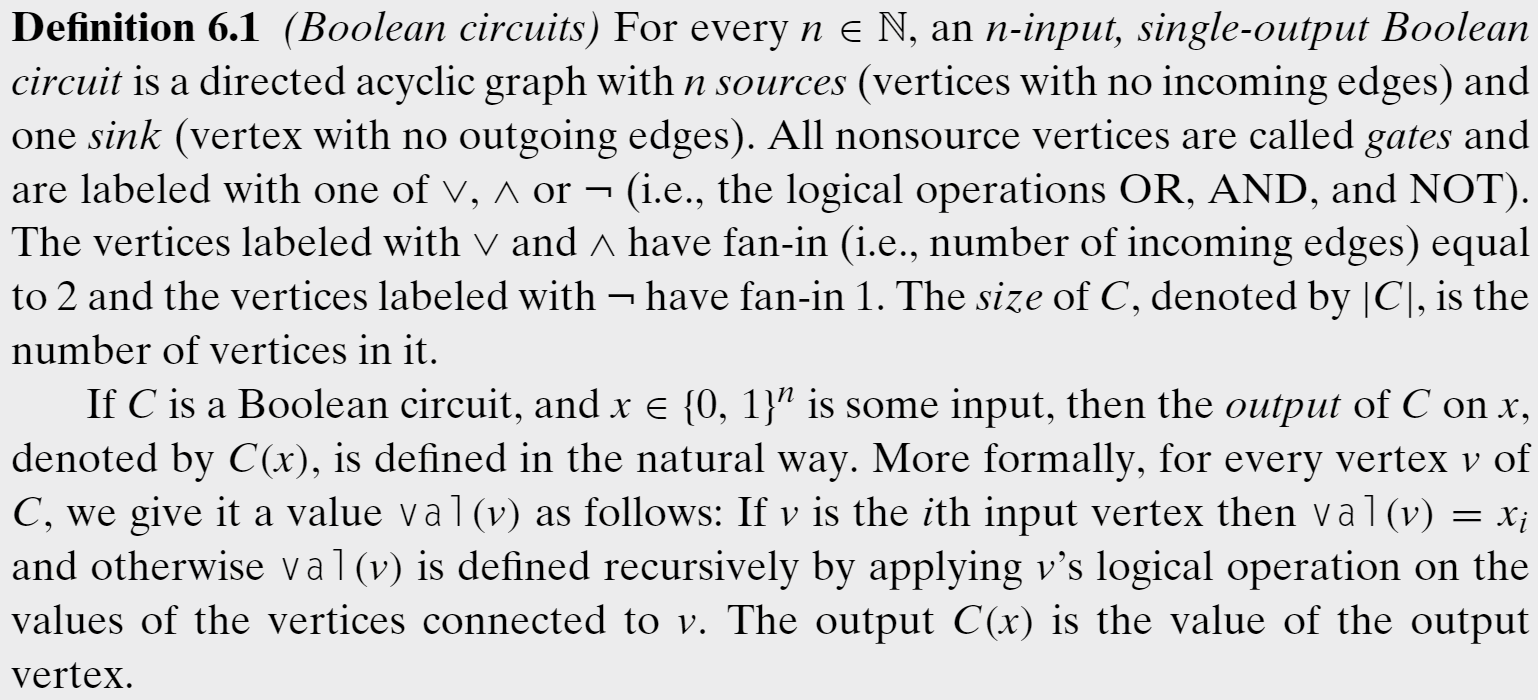
\includegraphics[width=0.9\linewidth]{../../5 & 6/note.assets/image-20210427143007226.png}
	\end{frame}
	
	\begin{frame}{电路族}
		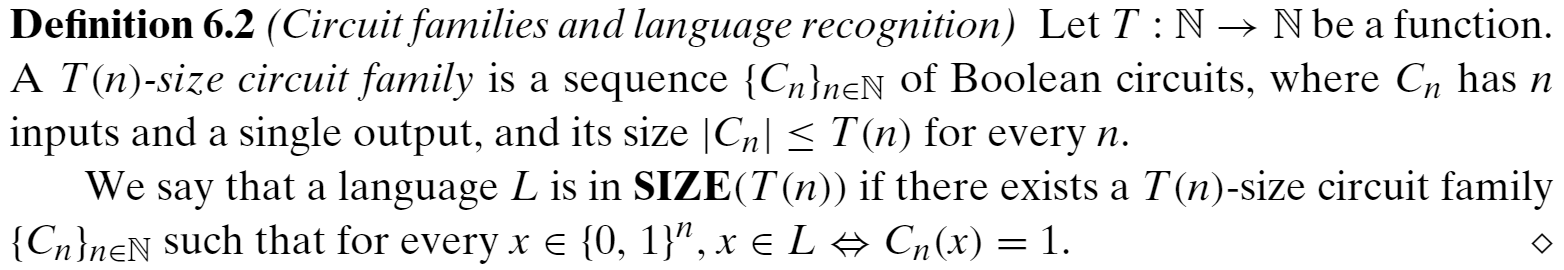
\includegraphics[width=\linewidth]{../../5 & 6/note.assets/image-20210427143311429.png}
	\end{frame}

	\begin{frame}{$\bf P_{/POLY}$:“小的电路”}
		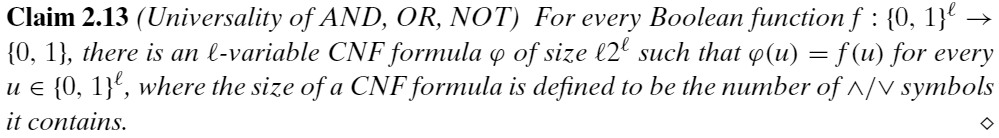
\includegraphics[width=\linewidth]{../../5 & 6/note.assets/image-20210427234507193.png}\newline
		
		因为 CNF 公式是电路的特殊形式,因此由 Claim 2.13 可以得到,每个由 $\{0,1\}^n$ 到 ${0,1}$ 的函数 $f$ 都可以由一个大小为 $n2^n$ 的布尔电路计算,但事实上,大小 $O(2^n/n)$ 足矣。考虑何为“小的电路”,可以定义:\newline
		
		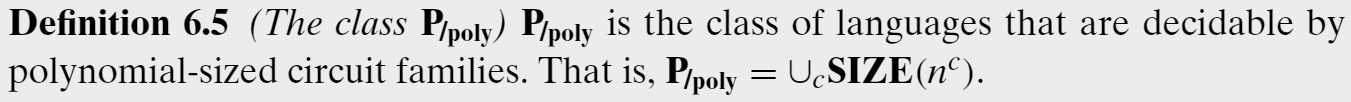
\includegraphics[width=\linewidth]{../../5 & 6/note.assets/image-20210427143807606.png}
		
		% 尽管多项式的次可能会很大,但是我们希望能够证明像 SAT 这样的语言不在 $\bf P_{/POLY}$ 中,当次尽可能大依然不能判定 SAT 语言时,这样的表述就会更强。
	\end{frame}

	\begin{frame}{$\bf P_{/POLY}$ 和 $\bf P$ 的关系}
		\begin{block}{Theorem 6.6}
			$\bf P\subseteq P_{/poly}$
		\end{block}
	
%		转移可以用电路表示,每一步都可以由多项式的电路完成,总共多项式步,组合可以得到一个仍为多项式大小的电路,根据输入计算最后的结果是否为 1。
%		
%		电路不仅可以是多项式大小的,还可以在多项式时间内计算,甚至在对数空间内计算(这里的空间与电路大小不同,我理解是可以用图灵机使用对数空间计算)。
		
		包含关系为真,存在不可判定的一元语言不属于 P,而每个一元语言都属于 $\bf P_{/poly}$
		
		\begin{block}{Claim 6.8}
			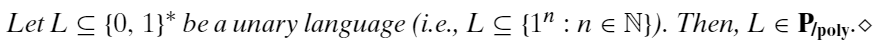
\includegraphics[width=0.8\linewidth]{../../5 & 6/note.assets/image-20210427235221740.png}
		\end{block}
	
		\begin{block}{UHALT}
			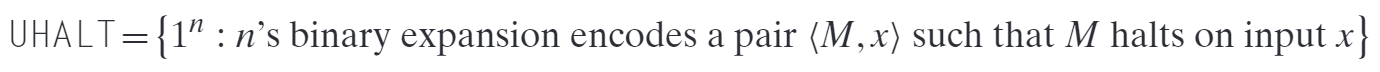
\includegraphics[width=\linewidth]{../../5 & 6/note.assets/image-20210427145209895.png}
		\end{block}
	\end{frame}

	\begin{frame}{电路可满足性}
		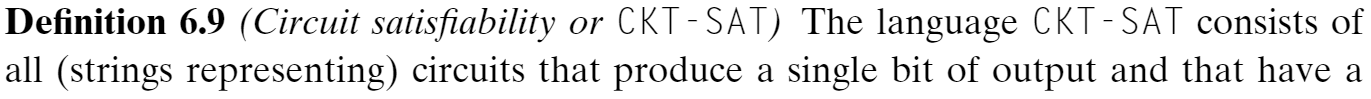
\includegraphics[width=\linewidth]{../../5 & 6/note.assets/image-20210427145455454.png}\newline
		
		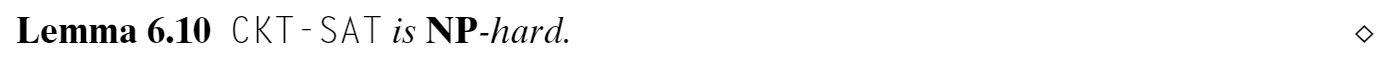
\includegraphics[width=\linewidth]{../../5 & 6/note.assets/image-20210427145611392.png}\newline
		
		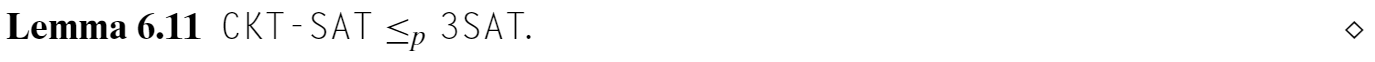
\includegraphics[width=\linewidth]{../../5 & 6/note.assets/image-20210427145621708.png}
	\end{frame}
	
	\section{一致生成的电路}
	\begin{frame}{$\bf P$-一致电路族}
		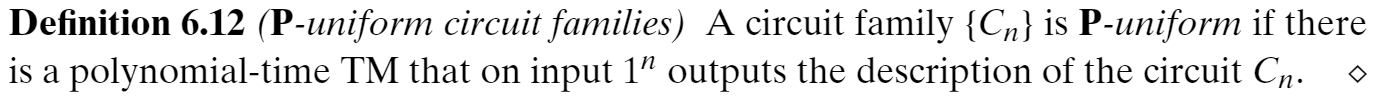
\includegraphics[width=\linewidth]{../../5 & 6/note.assets/image-20210427150551518.png}\newline
		
		$\bf P$-一致的限制使得 $\bf P_{/poly}$ 塌缩到了类 $\bf P$:\newline
		
		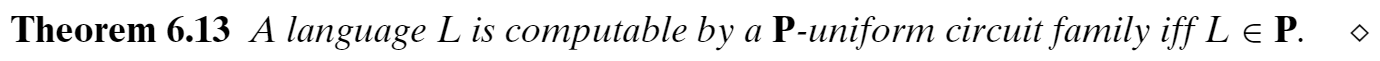
\includegraphics[width=\linewidth]{../../5 & 6/note.assets/image-20210427151158414.png}
	\end{frame}
	
	\begin{frame}{对数空间一致电路族}
		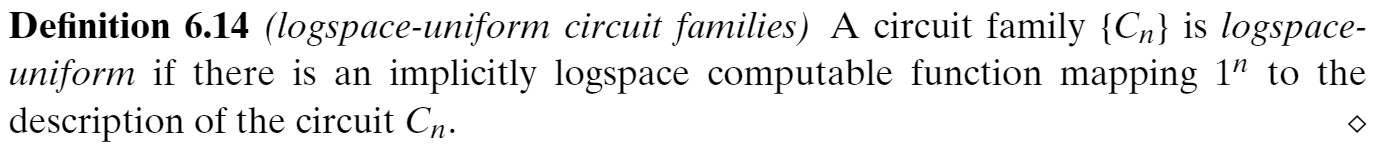
\includegraphics[width=\linewidth]{../../5 & 6/note.assets/image-20210427151635788.png}\newline
		
		因为对数空间的计算在多项式时间内进行,因此对数空间一致电路也是 $\bf P$-一致的。
	\end{frame}
	\begin{frame}
		表示一个大小为 S 的电路,可以用 S * S 的邻接矩阵和一个元素为节点标签的长度为 S 的数组表示。使用 [S] 中的数字标记每个顶点。一个电路族 $\{C_n\}$ 是对数空间一致的当且仅当以下函数可以在对数空间内计算:\newline
		
		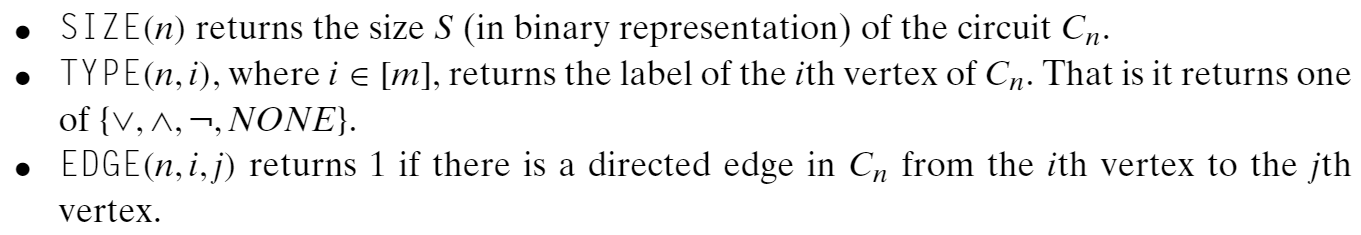
\includegraphics[width=\linewidth]{../../5 & 6/note.assets/image-20210427152140269.png}
	\end{frame}
	\begin{frame}
		对数空间一致同样使 $\bf P_{/poly}$ 塌缩到了 $\bf P$:\newline
		
		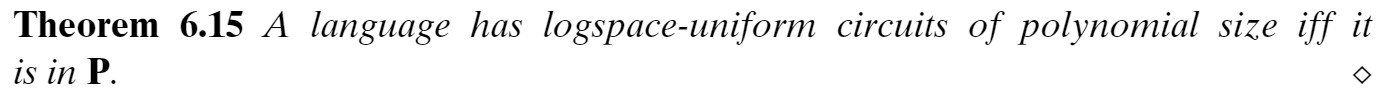
\includegraphics[width=\linewidth]{../../5 & 6/note.assets/image-20210427152252873.png}\newline
		
		我理解可以认为对数空间和多项式时间,都可以解决 P 类问题生成多项式大小的电路问题,并不能表示 $\bf L=P$。
	\end{frame}
	
	\section{接受建议的图灵机}
	\begin{frame}{接受建议的图灵机的定义}
		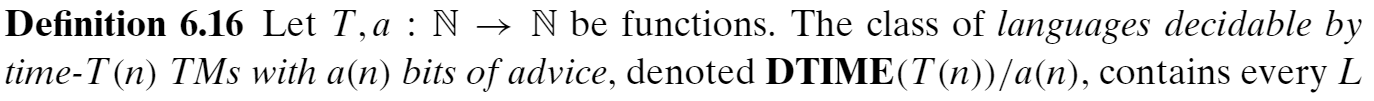
\includegraphics[width=\linewidth]{../../5 & 6/note.assets/image-20210427152508556.png}
	
		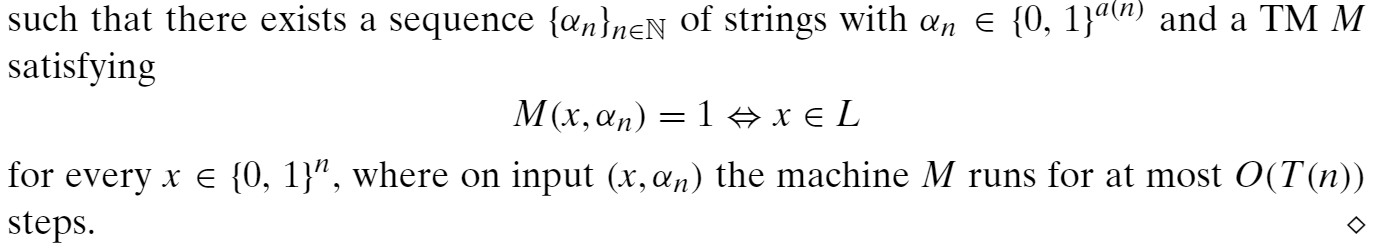
\includegraphics[width=\linewidth]{../../5 & 6/note.assets/image-20210427152516223.png}\newline
		
		比如对于 UHALT,对每个长度为 n 的输入,建议为 1 比特,表示输入是否为该语言的成员。
	\end{frame}

	\begin{frame}{再定义 $\bf P_{/poly}$}
		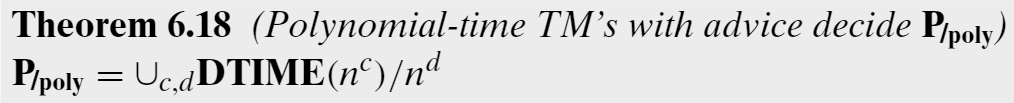
\includegraphics[width=\linewidth]{../../5 & 6/note.assets/image-20210427152742956.png}\newline
		
		建议相当于电路的描述,$n^c$ 则等价于允许电路的时间。
	\end{frame}
	
	\section{$\bf P_{/POLY}$ 和 $\bf NP$}
	\begin{frame}{$\bf P_{/POLY}$ 和 $\bf NP$}
		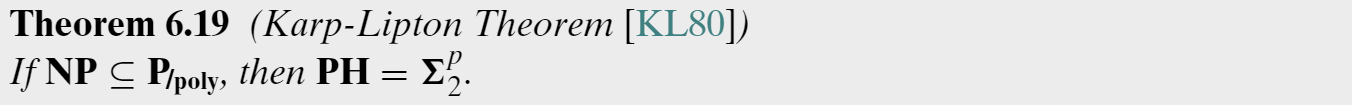
\includegraphics[width=\linewidth]{../../5 & 6/note.assets/image-20210427154847848.png}\newline
		
		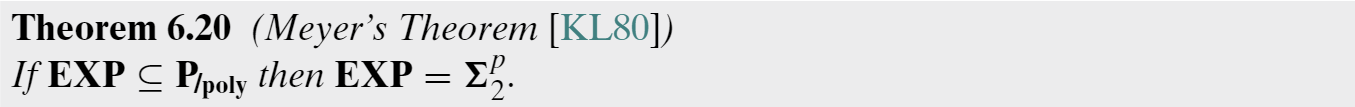
\includegraphics[width=\linewidth]{../../5 & 6/note.assets/image-20210427154857049.png}\newline
		
		Theorem 6.20 隐含着,如果 P = NP,则 EXP 不包含于 P/poly。因为如果 P = NP,则 P = $\Sigma_2^p$,若 EXP 包含于 P/poly,则 P = EXP,与时间分层定理矛盾。\newline
		
		"Thus upper bounds (in this case, $\bf NP\subseteq P$) can potentially be use dto prove circuit lower bounds"
	\end{frame}
	
	\section{电路下界}
	\begin{frame}{困难函数的存在}
		因为 P 包含于 P/poly,所以如果我们证明了 NP 不包含于 P/poly,就可以证明 $\bf P\neq NP$。\newline
		
		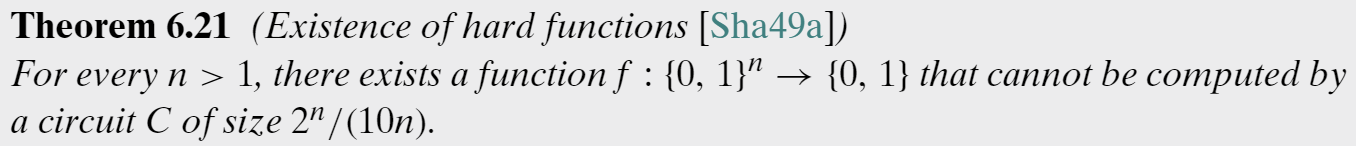
\includegraphics[width=\linewidth]{../../5 & 6/note.assets/image-20210427160637215.png}\newline
		
		因此只要找到一个这样的函数(不能被大于多项式大小的电路解决)是 NP 中的问题,就可以证明 NP 不包含与 P/poly,但是目前 NP 语言的最好的电路下界只有 $(5-o(1))n$。
	\end{frame}

	\section{非一致层级定理}
	\begin{frame}{非一致层级定理,Nonuniform Hierarchy Theorem}
		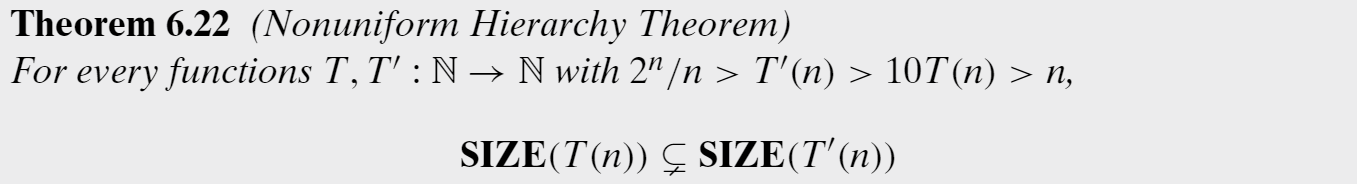
\includegraphics[width=\linewidth]{../../5 & 6/note.assets/image-20210427161541129.png}\newline
		
		可使用的电路大小增加,可以解决的问题增加。我理解这里的 10 是因为 6.21 中困难函数中的下界导致的,超过这个下界的函数不确定是否仍然是真子集关系。
	\end{frame}
	
	\section{电路类中更精细的分级}
	\begin{frame}{并行计算}
		并行计算机:$n$ 个处理器互联的网络,通信在 $O(log\ n)$ 步内完成。处理器在有锁的步(lock-step,全局同步的计步单位)内计算,且每步只完成计算的一小部分。\newline
		
		如果一个计算问题可以被一个使用 $n^{O(1)}$ 个处理器,在 $log^{O(1)}n$ 时间内运行的并行计算机解决,称它有一个高效的并行算法。
	\end{frame}

	\begin{frame}{类 $\bf NC$ 和 $\bf AC$}
		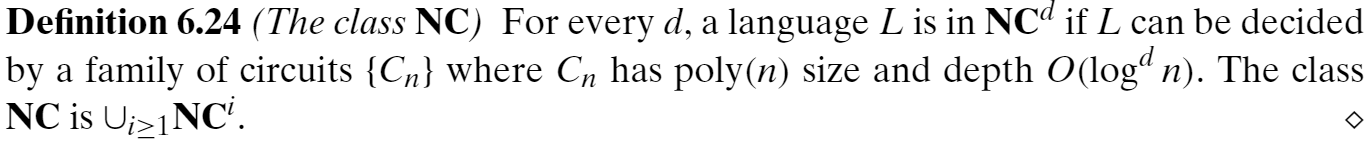
\includegraphics[width=\linewidth]{../../5 & 6/note.assets/image-20210427162533386.png}\newline
		
		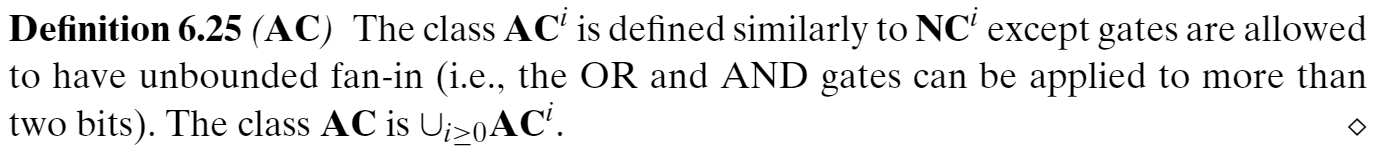
\includegraphics[width=\linewidth]{../../5 & 6/note.assets/image-20210427162543119.png}\newline
		
		$\bf NC$ 刻画了有高效并行算法的语言:
		
		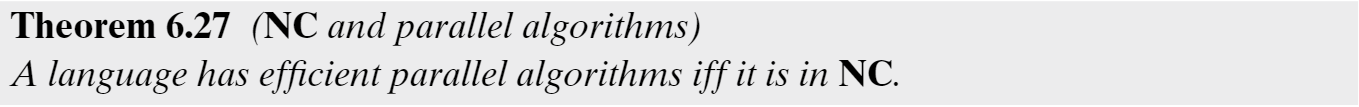
\includegraphics[width=\linewidth]{../../5 & 6/note.assets/image-20210427162618074.png}
	\end{frame}

	\begin{frame}{$\bf P$-完全性}
		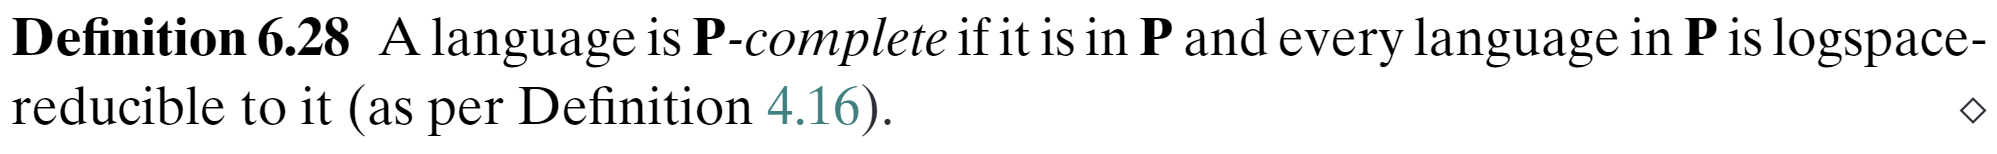
\includegraphics[width=\linewidth]{../../5 & 6/note.assets/image-20210427190230118.png}\newline
		
		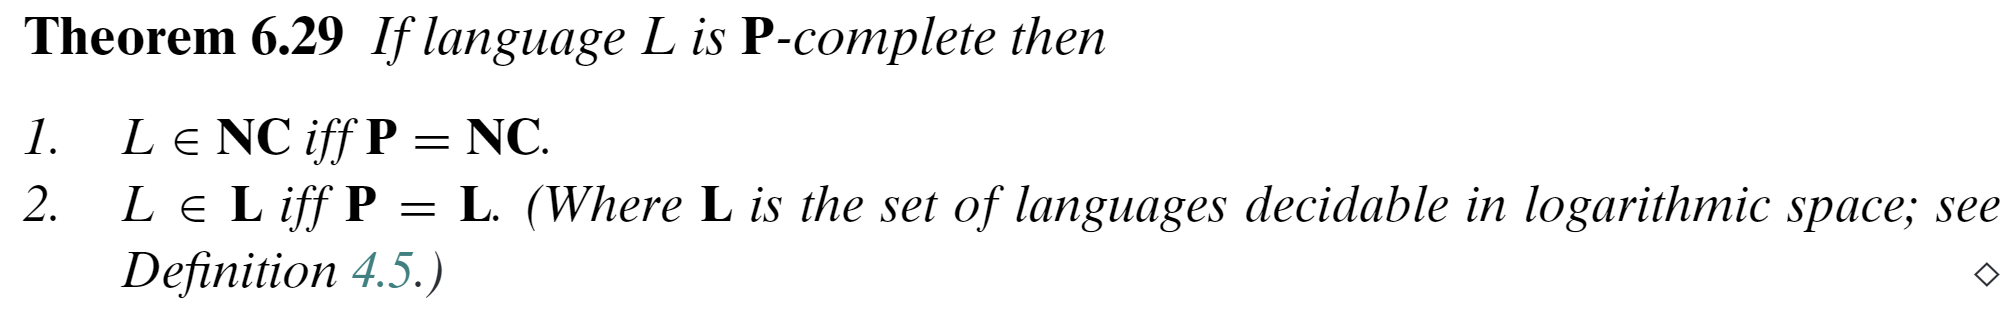
\includegraphics[width=\linewidth]{../../5 & 6/note.assets/image-20210427190510329.png}\newline
		
		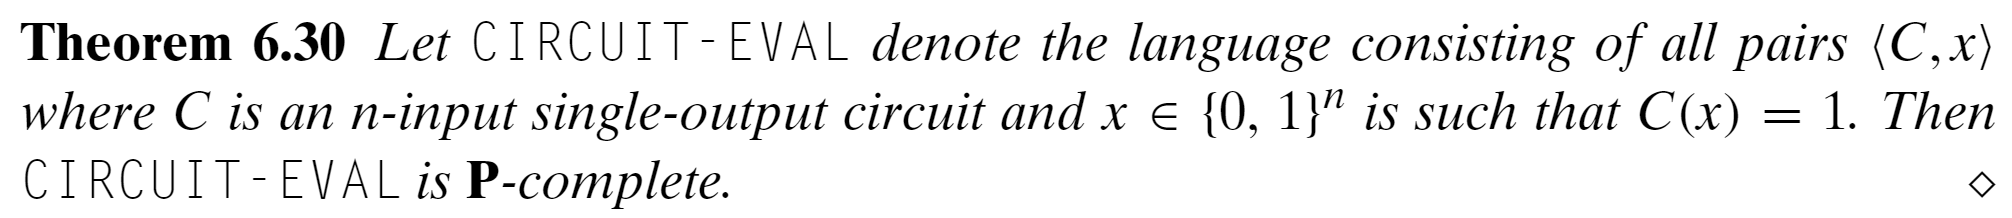
\includegraphics[width=\linewidth]{../../5 & 6/note.assets/image-20210427190538551.png}
	\end{frame}
	
	\section{指数大小的电路}
	\begin{frame}{DC一致}
		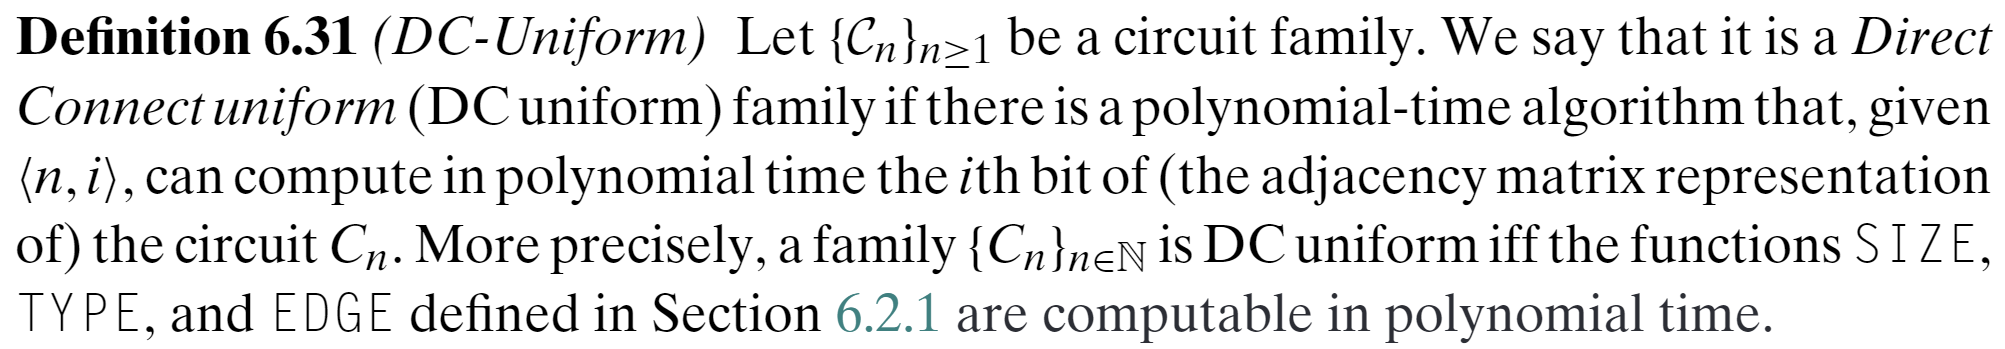
\includegraphics[width=\linewidth]{../../5 & 6/note.assets/image-20210427192246775.png}\newline
		
		对于任意语言,都有大小为 $O(2^n/n)$ 的电路可以解决。但实际中找到这样的电路可能非常困难。但我们可以加上一致条件,使得两个节点间是否连接可以多项式时间计算,也即 DC 的含义(我理解)。
		
%		类似指数空间一致族,将其中的隐式指数空间计算替换为多项式时间计算,得到的电路就可以达到指数大小,因为计算一位需要多项式步骤,枚举可以得到指数大小的可能。
	\end{frame}

	\begin{frame}{再定义 $\bf PH$ 类}
		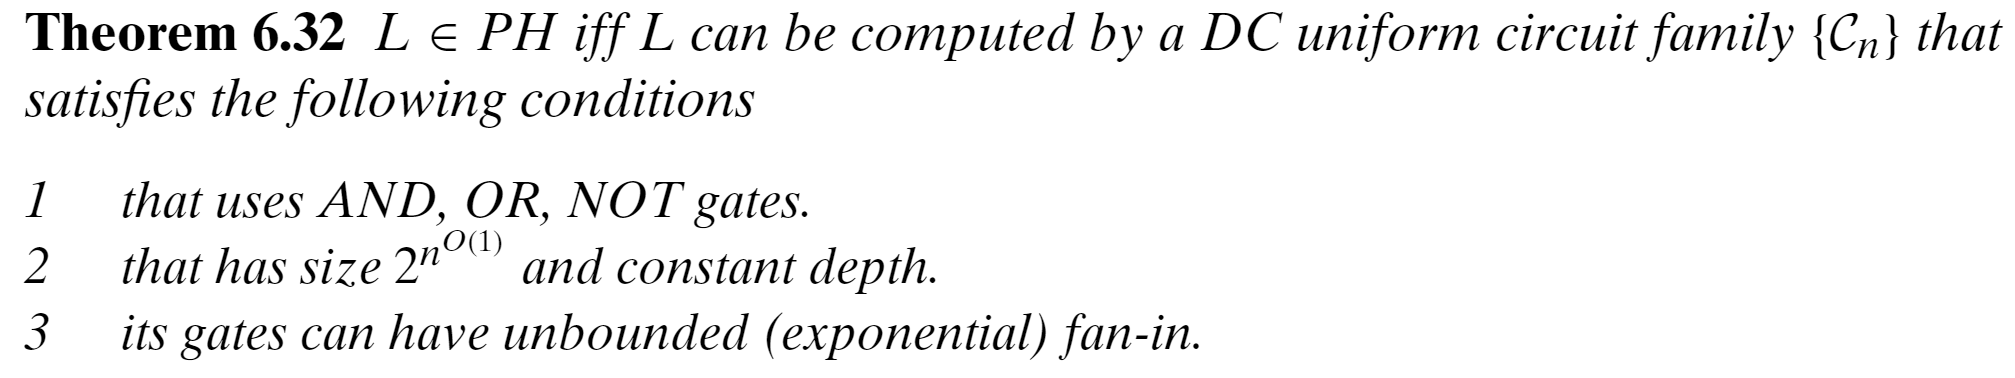
\includegraphics[width=\linewidth]{../../5 & 6/note.assets/image-20210427192410944.png}
		
		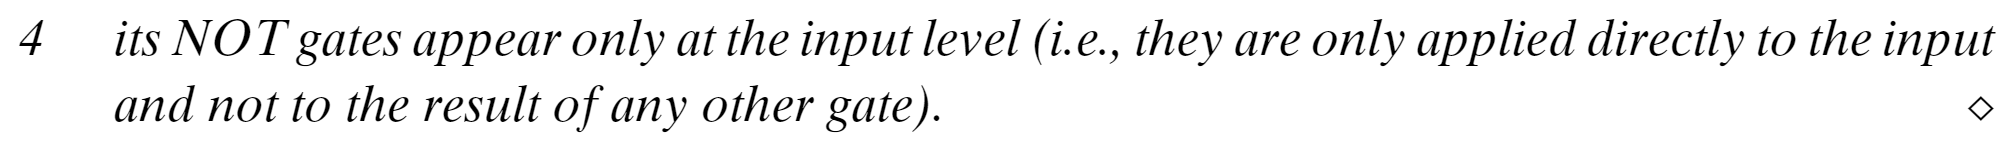
\includegraphics[width=\linewidth]{../../5 & 6/note.assets/image-20210427192420565.png}\newline
		
		% 我理解是前三条使得该类族可模拟 PH 问题中 $\forall$ 的选择,第四条使中间节点只能是 and/or,跟 PH 中的 $\forall$/$\exists$ 功能一致,而常数的深度和 PH 问题中不同的层次相对应。如果去掉常数深度的限制,则定义等价于 EXP。
	\end{frame}
	
\end{document}